% \subsection{Dataplane Offload}
\begin{table}[t]
\begin{scriptsize}
\begin{center}
\def\arraystretch{1.5}%  1 is the default, change whatever you need
\begin{tabular}{|p{1.8cm}|p{0.8cm}|p{0.8cm}|p{0.8cm}|}\hline 
% {\bf{Performance metric}} & {\bf{DPDK-based software UPF}} & {\bf{Dataplane offload}} & {\bf{Control plane offload}} \\ \hline 
 \multirow{2}{*}{\bf{UPF design}} &   \multicolumn{3}{c|}{\bf{Latency (in $\mu s$) with packet size}}  \\ %\hline
 & {\bf{64B}} & {\bf{IMIX}} & {\bf{1400B}} \\ \hline 
{\bf{SoftUPF}} & 138  & 176  & 294  \\ \hline
{\bf{DPOffload}}  & 130  & 140  & 222  \\ \hline
% {\bf{PartialDPOffload}} & Y & UL & 95 & 86  & 105 \\ \hline
% {\bf{FullDPOffload}} & Y & UL  & 80 & 68 &  67 \\ \hline
\end{tabular}
\setlength{\abovecaptionskip}{-8pt}
\setlength{\belowcaptionskip}{8pt}
\caption{SoftUPF vs. DPOffload: Dataplane latency.} 
\vspace{-1mm}
\label{tab:AvsC_latency}
\end{center}
\end{scriptsize}
\end{table}

\begin{table}[t]
\begin{scriptsize}
\begin{center}
\def\arraystretch{1.5}%  1 is the default, change whatever you need
\begin{tabular}{|p{3cm}|p{1.1cm}|p{1.2cm}|p{1.2cm}|}\hline 
% {\bf{Performance metric}} & {\bf{DPDK-based software UPF}} & {\bf{Dataplane offload}} & {\bf{Control plane offload}} \\ \hline 
{\bf{Performance metric}} & {\bf{SoftUPF}} & {\bf{DPOffload}} & {\bf{CPOffload}} \\ \hline 
{\bf{Throughput (messages/sec)}} & 5.1K  & 666  & 2.05M  \\ \hline
{\bf{Latency ($\mu s$)}} & 113  & 1646  & 26 \\ \hline
% {\bf{Performance per USD}} & 88  & 1 & 4.6K  \\ \hline
% {\bf{Performance per Watt}} & 40  & 1 & 41K \\ \hline
\end{tabular}
\setlength{\abovecaptionskip}{-8pt}
\setlength{\belowcaptionskip}{8pt}
\caption{Control plane performance.} 
\vspace{-2mm}
\label{tab:perf-cp-offload}
\end{center}
\end{scriptsize}
\end{table}
\noindent  {\textbf{Dataplane Offload.}} Next, we evaluate the benefits of offloading dataplane processing to programmable hardware by comparing the performance of the pure software UPF (\S\ref{sub:swUPF}) with one that offloads dataplane processing to a programmable NIC (\S\ref{sub:dpOffload}). We find that both designs saturate the 10Gbps linerate in our setup, and Table~\ref{tab:AvsC_latency} shows end-to-end latency measurements for the various traffic scenarios. As expected, dataplane offload improves latency by up to $24$\%.
%when all sessions send traffic within their rate limit. However, for scenario where 1\% of sessions send traffic beyond their specified AMBR, we find that SoftUPF and PartialDPOffload perform equally. If traffic has transient spikes and exceeds AMBR by small rate (up to 10\%), we find that FullDPOffload design improves latency by 18\% compared to SoftUPF.
% However, for scenario XX where 1\% of sessions send traffic beyond their specified AMBR, we find that XXX (fill suitable conclusion about userspace buffering). XXX: Also add a latency number for offlaoding of buffering in Design D. Some conclusion about how buffering is useful but must be worked out fully. 
\begin{figure}[t]
 \centering
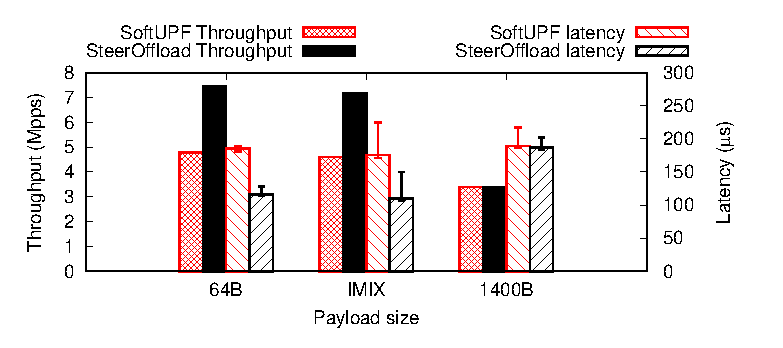
\includegraphics[width=0.45\textwidth]{graphs/pipelineVsRTT}
 \setlength{\abovecaptionskip}{4pt}
 \setlength{\belowcaptionskip}{-12pt}
 \caption{SoftUPF vs. SteerOffload: Performance.}
 %\vspace{-4mm}
 \label{fig:AvsB_tput}
\end{figure}

\begin{figure}[t]
    \centering
     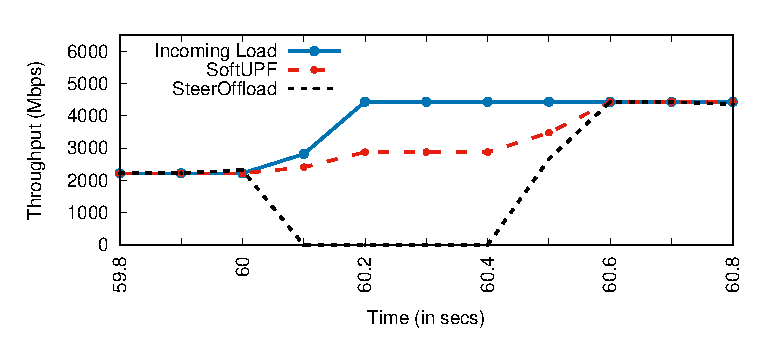
\includegraphics[width=0.4\textwidth]{graphs/dynScaling} % second figure itself
     \setlength{\abovecaptionskip}{4pt}
     \setlength{\belowcaptionskip}{-8pt}
 \caption{SoftUPF vs. SteerOffload: Dynamic scaling.}
 %\vspace{-4mm}
%  \caption{Dynamic Scaling.}
 \label{fig:AvsB_dyn_scl}
\end{figure}

\begin{figure}[t]
 \centering
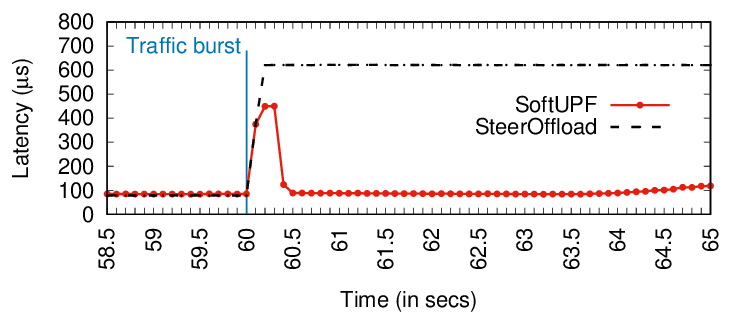
\includegraphics[width=0.4\textwidth]{graphs/heavyHitter}
 \setlength{\abovecaptionskip}{4pt}
 \setlength{\belowcaptionskip}{-8pt}
  \caption{SoftUPF vs. SteerOffload: Heavy hitters.}
  \vspace{-2mm}
%  \caption{SoftUPF vs SteerOffload: Heavy hitter redistribution.}
 \label{fig:AvsB_rebal}
\end{figure}

% \begin{table}[t]
% \begin{scriptsize}
% \begin{center}
% \def\arraystretch{1.5}%  1 is the default, change whatever you need
% \begin{tabular}{|p{1.8cm}|p{1.1cm}|p{0.6cm}|p{0.8cm}|p{0.8cm}|p{0.8cm}|}\hline 
% % {\bf{Performance metric}} & {\bf{DPDK-based software UPF}} & {\bf{Dataplane offload}} & {\bf{Control plane offload}} \\ \hline 
%  \multirow{2}{*}{\bf{UPF design}} &  \multirow{2}{*}{\bf{Over-}} & \multirow{2}{*}{\bf{UL:DL}} & \multicolumn{3}{c|}{\bf{Latency (in $\mu s$) with packet size}}  \\ %\hline
% & {\bf{subscribed}} & & {\bf{64B}} & {\bf{IMIX}} & {\bf{1400B}} \\ \hline 
% {\bf{SoftUPF}} & N & 1:2 & 138  & 176  & 294  \\ \hline
% {\bf{PartialDPOffload}} & N & 1:2 & 130  & 140  & 222  \\ \hline
% {\bf{PartialDPOffload}} & Y & UL & 95 & 86  & 105 \\ \hline
% {\bf{FullDPOffload}} & Y & UL  & 80 & 68 &  67 \\ \hline
% \end{tabular}
% \setlength{\abovecaptionskip}{-8pt}
% \setlength{\belowcaptionskip}{8pt}
% \caption{SoftUPF vs. DPOffload: Latency.} 
% \label{tab:AvsC_latency}
% \end{center}
% \end{scriptsize}
% \end{table}

% \begin{figure}[t]
%  \centering
% 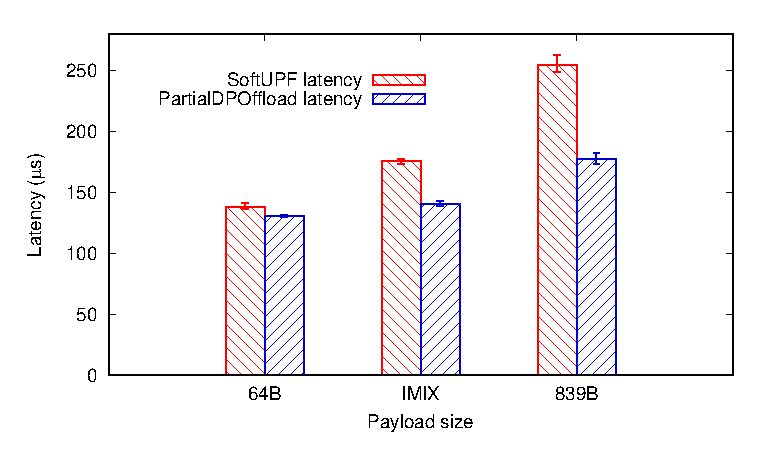
\includegraphics[width=0.4\textwidth]{graphs/SoftUPFVsPartialDPOffload}
%  \setlength{\abovecaptionskip}{4pt}
%  \setlength{\belowcaptionskip}{-12pt}
%  \caption{SoftUPF vs PartialDPOffload: Latency.}
%  \label{fig:AvsC_latency}
% \end{figure}

%
%\begin{table}[ht]
%\begin{scriptsize}
%\begin{center}
%\def\arraystretch{1.5}%  1 is the default, change whatever you need
%\begin{tabular}{|p{1cm}|p{1.2cm}|p{1.2cm}|}\hline 
%{\bf{}} & {\bf{Design A}} & {\bf{Design C}} \\ \hline 
%{\bf{Throughput (units/sec)}} & 22.52  & 47.44 \\ \hline
%{\bf{RTT latency (us)}} & 200 & 500\\ \hline
%% {\bf{Mpps per USD}} & 0.33  & 0.28 & 0.24  & 0.4 & 0.04  \\ \hline
%% {\bf{Mpps per Watt}} & 2.96 & 2.96 & 2.96 & 8.52 & 1.17 \\ \hline
%\end{tabular}
%% \setlength{\abovecaptionskip}{-5pt}
%% \setlength{\belowcaptionskip}{ 8pt}
%\caption{A vs C CP performance comparison.} 
%\label{tab:AvsC_cp_perf}
%\end{center}
%\end{scriptsize}
%\end{table}
%\\

%\\noindent \textbf{Cost/Power measurements:}
%\begin{table}[ht]
%\begin{scriptsize}
%\begin{center}
%\def\arraystretch{1.5}%  1 is the default, change whatever you need
%\begin{tabular}{|p{1cm}|p{1.2cm}|p{1.2cm}|}\hline 
%{\bf{}} & {\bf{Design A}} & {\bf{Design C}} \\ \hline 
%{\bf{Cost}} & 22.52  & 47.44 \\ \hline
%{\bf{Power}} & 200 & 500\\ \hline
%% {\bf{Mpps per USD}} & 0.33  & 0.28 & 0.24  & 0.4 & 0.04  \\ \hline
%% {\bf{Mpps per Watt}} & 2.96 & 2.96 & 2.96 & 8.52 & 1.17 \\ \hline
%\end{tabular}
%% \setlength{\abovecaptionskip}{-5pt}
%% \setlength{\belowcaptionskip}{ 8pt}
%\caption{A vs C cost \& power measurements} 
%\label{tab:AvsC_cost}
%\end{center}
%\end{scriptsize}
%\end{table}
%Table \ref{tab:AvsC_cost} compares the cost and power of both the designs.
%
%
%
